\documentclass[a4paper,french,12pt]{article}
\usepackage{geometry}
\geometry{a4paper, top=2cm, bottom=2.0cm, left=2.4cm, right=2.47cm}
\usepackage[frenchb]{babel}
\usepackage[utf8]{inputenc}
\usepackage[T1]{fontenc}
\usepackage{amsmath}
\usepackage{amssymb}
\usepackage{enumerate}
\usepackage{centernot}
\usepackage{multirow}
\usepackage{graphicx}
\usepackage{tikz}
\usetikzlibrary{positioning,calc,chains}
\def\P{\mathcal{P}}
\def\GUi{G \cup \{i\}}
\def\nottransition#1{\stackrel{#1}{\centernot\longrightarrow}}
\def\transition#1{\stackrel{#1}{\longrightarrow}}
\def\Transition#1{\stackrel{#1}{\Longrightarrow}}
\def\forte{\sim}
\def\observationnelle{\approx}
\def\conf{\ \text{conf}\ }
\DeclareMathOperator{\Tr}{Tr}
\DeclareMathOperator{\Acc}{Acc}
\DeclareMathOperator{\Ref}{Ref}
\def\si{\quad\text{si}\quad}
\let\simule\gtrsim
\let\simuleobs\gtrapprox
\let\estsimulepar\gtrsim
\begin{document}

\section{Files d'attente et équivalences}
\subsection{$B2err\simule B1$}

$B2err$ simule $B1$ car~:
\begin{itemize}
\item $B2err \simule B1$~:
  \begin{itemize}
  \item $B1\transition{inp} outp;B1$, et il existe $B2err\transition{inp}outp;B2err$.
  \item Il faut donc que $outp;B2err \simule outp;B1$.
  \end{itemize}
\item $outp;B2err \simule outp;B1$~:
  \begin{itemize}
  \item $outp;B1\transition{outp}B1$, et il existe $outp;B2err\transition{outp}B2err$.
  \item Il faut donc que $B2err \simule B1$, ce qui est notre premier point.
  \end{itemize}
\end{itemize}

\subsection{$\neg\ B2err\conf B1$}
$B2err$ n'est pas conforme à $B1$ car $Ref(B2err, inp) = \{\{inp\}, \{outp\}\}$, alors que $Ref(B1,inp) = \{\{outp\}\}$,
et donc on n'a pas $Ref(B2err, inp) \subseteq Ref(B1, inp)$.

\subsection{$B2par$ respecte-t-il la spécification $B_20$ ?}
$B2par$ respecte la spécification $B_20$~:
\begin{enumerate}[i)]
\item Un message émis a toujours été reçu : pour qu'un message soit
  émis par la porte $outp$ du $B1$ de droite, il faut qu'il ait été
  reçu par la porte $mid$ du $B1$ de droite, synchronisé sur la porte
  $mid$ du $B1$ de gauche. Pour que le message soit émis sur la porte
  $mid$ du $B1$ de gauche, il faut qu'il ait au préalable été reçu sur
  la porte $inp$ du $B1$ de gauche.
\item Lorsqu'un $B1$ reçoit un message, il refuse les $inp$ jusqu'à ce
  qu'il ait effectué un $outp$. Comme la porte $outp$ du $B1$ de
  gauche est synchronisée sur la porte $inp$ du $B1$ de droite, cela
  signifie que si les deux $B1$ «contiennent» un message, celui de
  droite n'accepera pas d'$inp$ tant qu'il n'aura pas effectué
  d'$outp$, et en cascade, celui de gauche ne pourra pas faire
  d'$outp$ tant que celui de droite n'aura pas été «vidé», et donc
  celui de gauche refusera les $inp$. On ne pourra donc pas effectuer
  un $inp$ sur le $B1$ de gauche tant que les deux $B1$ «contiendront»
  un message, et il ne pourra donc pas y avoir plus de deux messages
  dans la file.
\end{enumerate}

\subsection{$B2seq \observationnelle B2par$}

{\raggedright
  $B2seq$ et $B2par$ sont observationnellement équivalents car~:
  \begin{itemize}
  \item $B2s \observationnelle B2par$~:
    \begin{itemize}
    \item $B2s\transition{inp} B21$,
      et il existe $B2par \Transition{\hat{inp}} (i;B1[inp,i] \ |[i]|\ B1[i,outp])$
      et $B2par \Transition{\hat{inp}} (B1[inp,i] \ |[i]|\ outp;B1[i,outp])$.
    \item Dans l'autre sens,
      $B2par \transition{inp} (i;B1[inp,i] \ |[i]|\ B1[i,outp])$
      et il existe $B2s\transition{inp} B21$.
    \item Il faut donc que $B21 \observationnelle (i;B1[inp,i] \ |[i]|\ B1[i,outp])$.
    \end{itemize}
  \item $B21 \observationnelle (i;B1[inp,i] \ |[i]|\ B1[i,outp])$~:
    \begin{itemize}
    \item $B21 \transition{inp} outp;B21$,
      et il existe
      $(i;B1[inp,i] \ |[i]|\  B1[i,outp]) \Transition{\hat{inp}} (i;B1[inp,i] \ |[i]|\ outp;B1[i,outp])$
    \item $B21 \transition{outp} B2s$, et
      et il existe
      $(i;B1[inp,i] \ |[i]|\  B1[i,outp]) \Transition{\hat{outp}} (B1[inp,i] \ |[i]|\ B1[i,outp])$,
      autrement dit
      $(i;B1[inp,i] \ |[i]|\  B1[i,outp]) \Transition{\hat{outp}} B2par$
    \item Dans l'autre sens,
      $(i;B1[inp,i] \ |[i]|\ B1[i,outp]) \transition{i} (B1[inp,i] \ |[i]|\ outp;B1[i,outp])$,
      mais comme on $\hat{i}$ est le chemin vide, on n'aura rien à vérifier sur $B21$.
    \item Il faut donc que $outp;B21 \observationnelle (i;B1[inp,i] \ |[i]|\ outp;B1[i,outp])$,
      et que $B2s \observationnelle B2par$. Cette deuxième condition est en fait notre premier point.
    \end{itemize}
  \item $outp;B21 \observationnelle (i;B1[inp,i] \ |[i]|\ outp;B1[i,outp])$~:
    \begin{itemize}
    \item $outp;B21 \transition{outp}B21$,
      et il existe
      $(i;B1[inp,i] \ |[i]|\ outp;B1[i,outp]) \Transition{\hat{outp}} (i;B1[inp,i] \ |[i]|\ B1[i,outp])$.
    \item Il faut donc que $B21 \observationnelle (i;B1[inp,i] \ |[i]|\ B1[i,outp])$, ce qui est notre deuxième point.
    \end{itemize}
  \end{itemize}
}

\subsection{$B2ent = B2par$}

Étant donné que $B2ent$ et $B2par$ ne commencent pas par l'action
interne, tester leur égalité au sens de la congruence observationnelle
revient à tester s'ils sont observationnellement équivalents.

On applique donc la même méthode que dans la section précédente, avec
les équivalences suivantes~:

{\raggedright
  \begin{itemize}
  \item Pour que $B2ent = B2par$, il faut qu'après $inp$ (la seule
    action que les systèmes peuvent exécuter dans leurs états respectifs),
    $(outp;B1[inp;outp] ||| B1[inp;outp]) \observationnelle (i;B1[inp;i]\ |[i]|\ B1[i,outp])$.
  \item Pour cela, il faut qu'après $outp$,
    $(B1[inp;outp] ||| B1[inp;outp]) \observationnelle (B1[inp;i]\ |[i]|\ B1[i,outp])$,
    autrement dit $B2ent = B2par$, ce qui est une condition plus faible que le premier point.

    Il faut aussi qu'après $inp$,
    $(outp;B1[inp;outp] ||| outp;B1[inp;outp]) \observationnelle (i;B1[inp;i]\ |[i]|\ outp;B1[i,outp])$.
    
    Dans l'autre sens, on peut ignorer ce qui se passe après le $i$ de
    $(i;B1[inp;i]\ |[i]|\ B1[i,outp])$, car $\hat{i}$ est le chemin vide,
    donc pas de conditions sur $(outp;B1[inp;outp] ||| B1[inp;outp])$.
  \item Occupons-nous de
    $(outp;B1[inp;outp] ||| outp;B1[inp;outp]) \observationnelle (i;B1[inp;i]\ |[i]|\ outp;B1[i,outp])$.
    Dans ces états, les systèmes ne peuvent faire qu'$outp$. Il faut donc qu'après $outp$,
    $(outp;B1[inp;outp] ||| B1[inp;outp]) \observationnelle (i;B1[inp;i]\ |[i]|\ B1[i,outp])$,
    ce qui correspond au deuxième point.
  \end{itemize}
}

\subsection{$B2par \simuleobs B1$}

$B2par$ simule observationnellement $B1$ car~:

\begin{itemize}
\item $B1\transition{inp}outp;B1$, et il existe
  $B2par\Transition{\hat{inp}}(i;B1[inp,i]\ |[i]| B1[i;outp])$ et
  $B2par\Transition{\hat{inp}}(B1[inp,i]\ |[i]| outp;B1[i;outp])$.
  Il suffit donc que soit $(i;B1[inp,i]\ |[i]| B1[i;outp]) \simuleobs outp;B1$,
  soit $(B1[inp,i]\ |[i]| outp;B1[i;outp]) \simuleobs outp;B1$. On prend
\item On prend cette deuxième possibilité.
  $outp;B1 \transition{outp} B1$, et il existe
  $(B1[inp,i]\ |[i]| outp;B1[i;outp])\Transition{\hat{outp}}(B1[inp,i]\ |[i]| B1[i;outp])$,
  autrement dit
  $(B1[inp,i]\ |[i]| outp;B1[i;outp])\Transition{\hat{outp}}B2par$, notre premier point.
\end{itemize}

\subsection{$\not B2par \conf B1$}

Pour que $B2par$ soit conforme à $B1$, car pour toute trace $t$ de $B1$,
$\Acc(B2par) \subset\subset \Ref(B1)$.

\begin{itemize}
\item Pour la trace $\emptyset$, $\Acc(B2par) = \Acc(B1) = \{\{inp\}\}$.
\item Pour la trace $inp$, $\Acc(B2par) = \{\{\}, \{inp,outp\}\}$, mais $\Acc(B1) = \{\{outp\}\}$.
\item Pour la trace $inp;outp$, on est revenu aux mêmes états que la trace $\emptyset$.
\end{itemize}
Pour le point 2 $\forall X \in \{\{\}, \{inp,outp\}\},\quad \{outp\} \not\subseteq X$, et donc $\neg(B2par \conf B1)$

\section{Exercice de l'atelier}

\subsection{Question 1}

\begin{figure}[h]
  \centering
  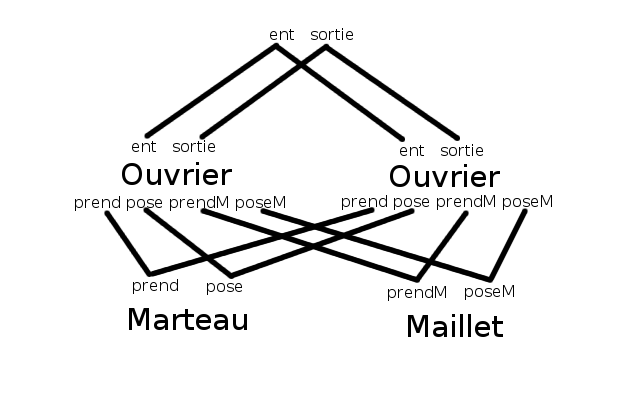
\includegraphics[width=15cm]{question1}
\end{figure}

\subsection{Question 2}

\begin{verbatim}
Maillet[prendM,poseM] := prendM;MailletOcc[prendM,poseM]
MailletOcc[prendM,poseM] := poseM;Maillet[prendM,poseM]
\end{verbatim}

\subsection{Question 3}

\begin{verbatim}
UtiliseMarteau[ent,sortie,prend,pose,prendM,poseM](travail:TRAVAIL) :=
  prend;sortie!fait(travail);pose;
  Ouvrier[ent,sortie,prend,pose,prendM,poseM]
\end{verbatim}

\begin{verbatim}
UtiliseMaillet[ent,sortie,prend,pose,prendM,poseM](travail:TRAVAIL) :=
  prendM;sortie!fait(travail);poseM;
  Ouvrier[ent,sortie,prend,pose,prendM,poseM]
\end{verbatim}

\begin{verbatim}
Commence[ent,sortie,prend,pose,prendM,poseM](travail:TRAVAIL) :=
  [facile(travail)] ->
    sortie!fait(travail);
    Ouvrier[ent,sortie,prend,pose,prendM,poseM]
  []
  [difficile(travail)] ->
    UtiliseMarteau[ent,sortie,prend,pose,prendM,poseM](travail)
  []
  [(not(facile(travail)) and not(difficile(travail)))] ->
    UtiliseOutil[ent,sortie,prend,pose,prendM,poseM](travail)
\end{verbatim}

\begin{verbatim}
Ouvrier[ent,sortie,prend,pose,prendM,poseM] :=
  ent?travail:TRAVAIL;
  Commence[ent,sortie,prend,pose,prendM,poseM](travail)
\end{verbatim}

\begin{verbatim}
Atelier[ent,sortie] :=
  hide prend,pose,prendM,poseM in
    (
      (
        Marteau[prend,pose]
        |||
        Maillet[prendM,poseM]
      )
      |[prend,pose,prendM,poseM]|
      (
        Ouvrier[ent,sortie,prend,pose,prendM,poseM]
        |||
        Ouvrier[ent,sortie,prend,pose,prendM,poseM]
      )
    )
\end{verbatim}

\subsection{Question 4}

Nécessite l'outil \verb!casear!.

\subsection{Question 5}

\begin{verbatim}
AtelierV[ent,sortie] :=
  hide e,s in
    Verificateur[ent,sortie,e,s]
    |[e,s]|
    Atelier[e,s]
\end{verbatim}

La composition parallèle générale synchronisant les ouvriers et le
vérificateur est la synchronisation sur l'ensemble de portes
$\{ent,sortie\}$ de l'atelier sans vérificateur.

On place le vérificateur «entre» les ouvriers et l'environnement~: Si
un travail est mal fait, le vérificateur le défait et le repasse à
l'entrée des ouvriers, sinon, il l'envoie vers la sortie de
l'environnement. À tout moment, il peut récupérer du travail depuis
l'environnement, et le passer aux ouvriers. Nous avons choisi de ne
pas limiter le nombre de fois que le vérificateur peut laisser les
ouvriers obtenir du travail depuis l'environnement, puisque nous ne
savons pas combien de travaux peuvent être sur les tapis roulants
$ent$ et $sortie$ sans que le vérificateur y ait encore eu accès.

\begin{verbatim}
Verificateur[ent,sortie,e,s] :=
  (
    s?produit:PRODUIT;
    [not(correct(produit))] ->
      e!defait(produit);Verificateur[ent,sortie,e,s]
    []
    [correct(produit)] ->
      sortie!produit;Verificateur[ent,sortie,e,s]
  )
  []
  (
    ent?travail:TRAVAIL;
    e!travail;
    Verificateur[ent,sortie,e,s]
  )
\end{verbatim}

\subsection{Question 6}

$Assemble$ n'est pas observationnellement équivalent à $Atelier$, car
après avoir exécuté l'action $ent$, $Atelier$ peut encore exécuter
$ent$ (puisqu'il y a deux ouvriers, qui peuvent accepter deux
travaux), tandis que $Assemble$ ne pourra exécuter que $sortie$.

{\raggedright
  \begin{itemize}
  \item $Atelier[\dots] \transition{ent} (\dots) \ |[\dots]|\ (Commence[\dots] ||| Ouvrier[\dots])$,
    et il existe
    $Assemble[\dots] \transition{ent} Assembler[\dots]$. Il faudrait que 
    $(\dots) \ |[\dots]|\ (Commence[\dots] ||| Ouvrier[\dots]) \observationnelle Assembler[\dots]$.
  \item Mais
    $(\dots) \ |[\dots]|\ (Commence[\dots] ||| Ouvrier[\dots]) \not\observationnelle Assembler[\dots]$
    car $(\dots) \ |[\dots]|\ (Commence[\dots] ||| Ouvrier[\dots]) \transition{ent} (\dots) \ |[\dots]|\ (Commence[\dots] ||| Commence[\dots])$
    tandis que $Assembler[\dots] \nottransition{ent}$.
  \end{itemize}
}
\subsection{Question 7}

Nécessite l'outil \verb!aldebaran!.

\end{document}
